En el siglo XX nace la teoría de autómatas como siguiente nivel de conceptualización sobre qué son las máquinas y qué pueden hacer, la pregunta fundamental de este momento histórico es: ¿Qué problemas puede resolver una máquina?.

\vspace{10px}

Daremos ahora una definición de autómata alejada del mecanicismo anterior, más parecido al modelo abstracto de las álgebras de Boole: Un autómata finito es una máquina (abstracta) cuya salida no depende solo de la entrada actual.

\vspace{10px}

Un autómata finito tiene estados, posiciones de memoria que dependerán de las entradas anteriores, esto eleva la capacidad expresiva del autómata muy por encima de la del S.C. \\

- En electrónica un autómata es un sistema secuencial, aunque en ocasiones la palabra es utilizada también para referirse a un robot. [...] Sin embargo, la rápida evolución de los autómatas hace que esta definición no esté cerrada. (Wikipedia)- \\

Aquí un sistema secuencial es justo lo que hemos definido como autómata, un sistema combinacional dotado de memoria.  Un ejemplo muy sencillo de un cálculo que podría hacerse con un autómata finito y no bastaría con un sistema combinacional, sería la tarea de decidir si un conjunto de ceros es par o impar. Esto puede parecer una tarea trivial pero es un cálculo recurrente en la comprobación de errores de protocolos de comunicación tan conocidos como el TCP/IP, que implementan un bit de paridad para este fin.

\vspace{10px}


Definiremos qué es un autómata con más rigurosidad en lo que sigue, pero por ahora, daremos un ejemplo de lo que será un autómata bajo el formalismo que plantearemos. El robot WATBOT1 tenía una interfaz conversacional implementada, pues bien, dicha interfaz se modelaba mediante un autómata finito. Es decir: El robot en sí no era el autómata, el mecanismo que le permitía dialogar (aunque fuese de manera precaria) se modeló con una máquina de estado finito.

\subsubsection{Aumentando la abstracción: Lenguajes y problemas }


Esta evolución sobre lo que era una máquina y qué problemas podía resolver planteó el mismo problema que habíamos subrayado antes. Si podemos clasificar las máquinas que tenemos según su complejidad, ¿podríamos hacerlo con los problemas?

\vspace{10px}

Este es fundamentalmente el objeto de estudio de la teoría de autómatas, pues responde fundamentalmente a la pregunta: ¿Qué máquina necesito para resolver este problema?

\vspace{10px}

La definición del lenguaje formal como se hace en esta teoría es bastante natural:

\vspace{10px}


Sea  $\mathcal{A}$ un conjunto finito de símbolos, a este conjunto lo llamaremos alfabeto, muy en consonancia con el uso popular del concepto. A los símbolos de $\mathcal{A}$ se les llamará letras, a las secuencias finitas de letras, palabras, y a todas las palabras que se puedan formar con las letras se las conoce como lenguaje generado por $\mathcal{A}$ o por sintetizar: $\mathcal{A}^{*}$. Un lenguaje sobre $\mathcal{A}$, será un subconjunto de su lenguaje generado. Esto es:


$$ \mathcal{L} \text{ es un lenguaje sobre } \mathcal{A}  \iff \mathcal{L} \subset \mathcal{A^{*}} $$


Hasta aquí existe un paralelismo evidente con lo que asociaríamos con un lenguaje de manera popular. Pues bien, existe una relación entre las categorías de complejidad que mencionamos antes y los lenguajes. \\


Por ejemplo, definamos el siguiente lenguaje, palabras sobre $\{0,1\}$ tales que tengan un número par de 0's.

\begin{equation}
\mathcal{L} = \{\omega \in \{0,1\}^{*} : \text{ $\omega$ tiene un nº par de 0's} \}
\end{equation}


\begin{center}
	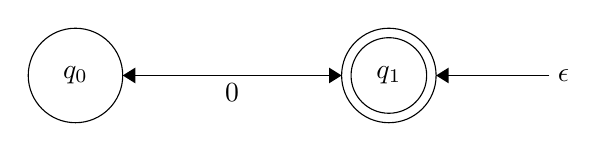
\begin{tikzpicture}[scale=0.2]
	\tikzstyle{every node}+=[inner sep=0pt]
	\draw [black] (40.6,-19.3) circle (3);
	\draw (40.6,-19.3) node {$q_1$};
	\draw [black] (40.6,-19.3) circle (2.4);
	\draw [black] (20.7,-19.3) circle (3);
	\draw (20.7,-19.3) node {$q_0$};
	\draw [black] (37.6,-19.3) -- (23.7,-19.3);
	\fill [black] (23.7,-19.3) -- (24.5,-19.8) -- (24.5,-18.8);
	\draw [black] (23.7,-19.3) -- (37.6,-19.3);
	\fill [black] (37.6,-19.3) -- (36.8,-18.8) -- (36.8,-19.8);
	\draw (30.65,-19.8) node [below] {$0$};
	\draw [black] (50.8,-19.3) -- (43.6,-19.3);
	\draw (51.3,-19.3) node [right] {$\epsilon$};
	\fill [black] (43.6,-19.3) -- (44.4,-19.8) -- (44.4,-18.8);
	\end{tikzpicture}
\end{center}

%TODO citar el libro que has sacado de la biblioteca

El siguiente autómata sería capaz de clasificar las palabras sobre el lenguaje generado por $\{0,1\}^{*}$ de manera que podría decirnos qué palabras pertenecen exactamente al lenguaje. La correspondencia entre lenguaje y autómata es aún mayor, porque de hecho, este autómata sólo acepta las palabras del lenguaje $\mathcal{L}$. Una vez introducidos los conceptos daremos una definición rigurosa.

\vspace{10px}

Un autómata se modela de la siguiente manera, es una tupla de 5 elementos: $(Q, \mathcal{A}, q_0, \delta, F)$

\begin{itemize}
	\item $Q$ : Conjunto finito de estados que numeramos $ q_0 \dots q_n$
	\item $\mathcal{A}$: Alfabeto, conjunto finito de símbolos sobre el que se crearán palabras del lenguaje.
	\item $q_0$ El estado inicial.
	\item $\delta :Q\times \mathcal{A} \rightarrow Q$. Función que nos indica cómo leer la palabra.
	\item $F$ : Conjunto de estados finales
\end{itemize}


Explicaremos ahora con detenimiento la relación entre los lenguajes y los autómatas pues son dos maneras de hablar del mismo concepto. Supongamos el siguiente lenguaje sobre $\{0,1\}$: Si la palabra empieza por 1 no pertenece al lenguaje, si empieza por 0 sí. El autómata que únicamente acepta las palabras de este lenguaje es el siguiente:

\begin{center}
	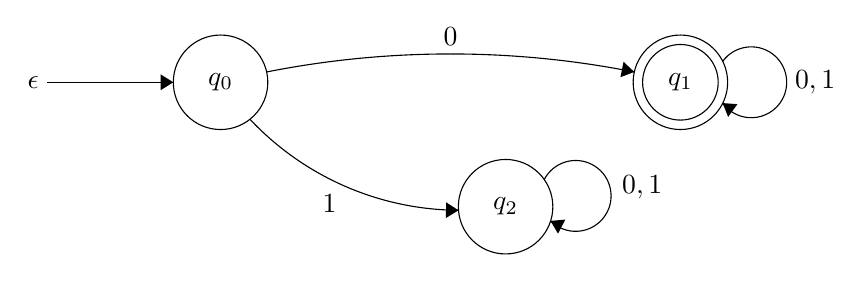
\begin{tikzpicture}[scale=0.2]
	\tikzstyle{every node}+=[inner sep=0pt]
	\draw [black] (20.6,-27.7) circle (3);
	\draw (20.6,-27.7) node {$q_0$};
	\draw [black] (49.8,-27.7) circle (3);
	\draw (49.8,-27.7) node {$q_1$};
	\draw [black] (49.8,-27.7) circle (2.4);
	\draw [black] (38.7,-35.6) circle (3);
	\draw (38.7,-35.6) node {$q_2$};
	\draw [black] (23.527,-27.044) arc (101.19936:78.80064:60.1);
	\fill [black] (46.87,-27.04) -- (46.19,-26.4) -- (45.99,-27.38);
	\draw (35.2,-25.4) node [above] {$0$};
	\draw [black] (52.48,-26.377) arc (144:-144:2.25);
	\draw (57.05,-27.7) node [right] {$0,1$};
	\fill [black] (52.48,-29.02) -- (52.83,-29.9) -- (53.42,-29.09);
	\draw [black] (35.712,-35.827) arc (-90.34893:-136.81015:18.322);
	\fill [black] (35.71,-35.83) -- (34.92,-35.32) -- (34.91,-36.32);
	\draw (27.52,-34.81) node [below] {$1$};
	\draw [black] (41.148,-33.885) arc (152.74451:-135.25549:2.25);
	\draw (46.07,-34.38) node [right] {$0,1$};
	\fill [black] (41.55,-36.5) -- (42.03,-37.31) -- (42.49,-36.42);
	\draw [black] (9.6,-27.7) -- (17.6,-27.7);
	\draw (9.1,-27.7) node [left] {$\epsilon$};
	\fill [black] (17.6,-27.7) -- (16.8,-27.2) -- (16.8,-28.2);
	\end{tikzpicture}
\end{center}



Un autómata puede presentarse también a modo de grafo como vemos, los estados se representan como nodos y los arcos representan las transiciones que modela la función $\delta(\cdot)$. Leemos la palabra de izquierda a derecha y por cada símbolo de la palabra, buscamos cuál es la transición asociada al estado en que nos encontramos y el símbolo que estamos leyendo.

\vspace{10px}

Ahora bien, uno de los estados está marcado con dos circunferencias, este es un estado final, al ser el único: $F = \{q_1\}$. El resto de los elementos de la tupla serían:

\begin{multicols}{2}
	\begin{itemize}
		\item $Q =\{q_0,q_1,q_2\}$
		\item $\mathcal{A} = \{0,1\}$
		\item $F = \{q_1\}$
	\end{itemize}

\end{multicols}

En cuanto a la función de transición, tendremos que el par $(a,q_i)$ pertenece al dominio de la función, si en el grafo existe un arco que salga de $q_i$ con etiqueta $a$. Las transiciones serían las siguientes:

\begin{multicols}{2}
	\begin{itemize}
		\item $\delta(0,q_0)=q_1$
		\item $\delta(1,q_0)=q_2$
		\item $\delta(a,q_1)=q_1 \ \forall a \in \{0,1\}$
		\item $\delta(a,q_2)=q_2 \ \forall a \in \{0,1\}$
	\end{itemize}
\end{multicols}

El símbolo $\epsilon$ se reserva para la palabra vacía, una entelequia que simboliza la palabra que no contiene ninguna letra.





\subsubsection{No-Determinismo}

Los autómatas que hemos examinado antes son deterministas, es decir, dada una entrada y partiendo de un estado, es trivial averiguar en qué estado acabaremos una vez leída esta. Sin embargo podemos considerar qué pasaría si nuestra función define las siguientes transiciones:

\begin{multicols}{2}
	\begin{itemize}
		\item $\delta(0,q_i)=q_j$
		\item $\delta(0,q_i)=q_k \hspace{2cm} j\neq k$
	\end{itemize}
\end{multicols}


Es decir: ¿Qué hacemos si estando el estado $q_i$ leemos un $0$? ¿Nos vamos a $q_j$ o a $q_k$? La respuesta no es simple. Los autómatas finitos no deterministas nacen por su enorme capacidad de expresión y su definición menos rigurosa que la de los anteriores. Sería una gran ventaja que fuesen equivalente, de manera que pudiésemos usar este último, más sencillo de definir, y aun así tener la potencia expresiva del anterior. La respuesta será que sí.

\vspace{10px}


Su definición es parecida a la anterior salvo por un detalle, la función de transición:

\vspace{0.20cm}

$$\delta :Q\times \mathcal{A} \rightarrow \mathcal{P}(Q)$$

\vspace{0.3cm}

Aquí $\mathcal{P}(Q)$ es el conjunto potencia de $Q$, las partes de $Q$, es decir, dado un estado y un símbolo, podemos construir un autómata que tenga una arco conectando este estado $q_i$ con todos los demás incluyendo el mismo.



\newpage

Supongamos el siguiente problema, queremos crear un autómata que nos distinga  si una palabra pertenece a este lenguaje:

$$\{ \omega \in \{0,1\}^* : \omega \text{ tiene un número par de 0's} \} \cup \{\omega  \in \{0,1\}^*: \omega \text{ contiene al cadena }  101 \}$$

\begin{center}
	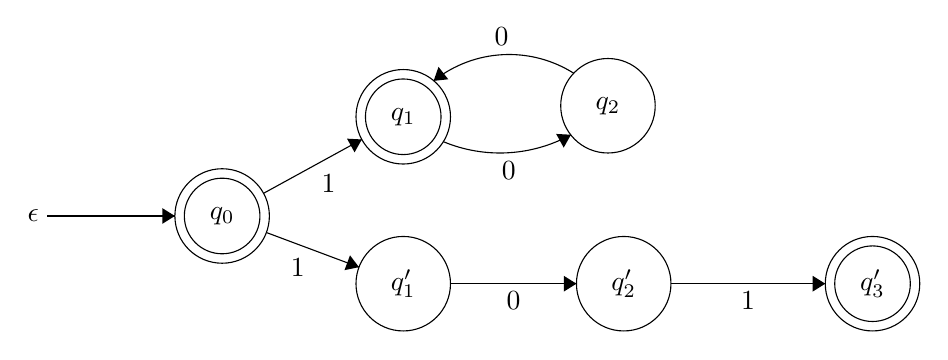
\begin{tikzpicture}[scale=0.2]
	\tikzstyle{every node}+=[inner sep=0pt]
	\draw [black] (17.2,-29) circle (3);
	\draw (17.2,-29) node {$q_0$};
	\draw [black] (17.2,-29) circle (2.4);
	\draw [black] (28.7,-22.7) circle (3);
	\draw (28.7,-22.7) node {$q_1$};
	\draw [black] (28.7,-22.7) circle (2.4);
	\draw [black] (28.7,-33.3) circle (3);
	\draw (28.7,-33.3) node {$q_1'$};
	\draw [black] (41.7,-22) circle (3);
	\draw (41.7,-22) node {$q_2$};
	\draw [black] (42.7,-33.3) circle (3);
	\draw (42.7,-33.3) node {$q_2'$};
	\draw [black] (58.5,-33.3) circle (3);
	\draw (58.5,-33.3) node {$q_3'$};
	\draw [black] (58.5,-33.3) circle (2.4);
	\draw [black] (6.1,-29) -- (14.2,-29);
	\draw (5.6,-29) node [left] {$\epsilon$};
	\fill [black] (14.2,-29) -- (13.4,-28.5) -- (13.4,-29.5);
	\draw [black] (19.83,-27.56) -- (26.07,-24.14);
	\fill [black] (26.07,-24.14) -- (25.13,-24.09) -- (25.61,-24.96);
	\draw (23.95,-26.35) node [below] {$1$};
	\draw [black] (20.01,-30.05) -- (25.89,-32.25);
	\fill [black] (25.89,-32.25) -- (25.32,-31.5) -- (24.97,-32.44);
	\draw (22.01,-31.67) node [below] {$1$};
	\draw [black] (39.348,-23.841) arc (-61.15181:-112.68383:9.343);
	\fill [black] (39.35,-23.84) -- (38.41,-23.79) -- (38.89,-24.66);
	\draw (35.4,-25.54) node [below] {$0$};
	\draw [black] (31.7,-33.3) -- (39.7,-33.3);
	\fill [black] (39.7,-33.3) -- (38.9,-32.8) -- (38.9,-33.8);
	\draw (35.7,-33.8) node [below] {$0$};
	\draw [black] (45.7,-33.3) -- (55.5,-33.3);
	\fill [black] (55.5,-33.3) -- (54.7,-32.8) -- (54.7,-33.8);
	\draw (50.6,-33.8) node [below] {$1$};
	\draw [black] (30.625,-20.424) arc (128.5933:57.57106:7.686);
	\fill [black] (30.63,-20.42) -- (31.56,-20.32) -- (30.94,-19.53);
	\draw (34.95,-18.21) node [above] {$0$};
	\end{tikzpicture}
\end{center}

Si nos fijamos, los estados $q_i'$ y los $q_i'$ conforman 2 autómatas independientes, que hemos unido usando el no-determinismo en la transición $\delta(q_0,1)$ hemos dado un autómata que reconoce únicamente las palabras del lenguaje unión, uniendo los autómatas.

\vspace{10px}

Esto se puede extender todavía más, introduciendo el concepto de las transiciones nulas. Una transición nula es la manera más cómoda de unir dos autómatas pues puedes moverte por libertad por todos los estados entre los que haya una transición nula. Intuitivamente esto quiere decir que podemos ir de un estado a otro sin leer el símbolo actual.


\subsubsection{Ejemplos de Autómatas}

Después de estas consideraciones, queda pensar cuál es el papel de estos modelos en cuanto a su papel en temas de robótica. Pues pensemos en una función relativamente simple que querríamos que tuviese un robot, la comunicación por ejemplo.

\vspace{10px}

Un protocolo de comunicación es de los requerimientos más fundamentales, ya no en la robótica sino en cualquier sistema de relativa complejidad pues la función en sí es tan importante como la existencia de una interfaz de comunicación con el beneficiario de la función a implementar. No nos referimos necesariamente a la capacidad de expresión del agente, sino a la existencia de un protocolo que le permita transmitir información de forma coherente y exacta con el humano con el que interaccione, aunque este sea su programador.

\vspace{10px}

Hablamos por ejemplo de la implementación del protocolo TCP/IP, que en el fondo, es una máquina de estados finita o como lo venimos llamando: un autómata finito determinista. Daremos un ejemplo de cómo modelar un sistema de autenticación de usuarios con una máquina de estados muy simple.

\begin{itemize}
	\item $q_0$ Estado Inicial: En espera
	\item $F=\{q_1\}$ Único estado final : Autentificado
	\item $\mathcal{A}=\{001,010,011,000\}$
\end{itemize}

En cuanto a la función de transición. Supongamos que nuestro sistema incorpora la siguiente directivas:

\begin{multicols}{2}
	\begin{itemize}
		\item Envío de contraseña incorrecta: $001$
		\item Envío de contraseña correcta: $010$
		\item Salir: $011$
		\item Error: $000$
	\end{itemize}
\end{multicols}

\vspace{1cm}

\begin{center}
	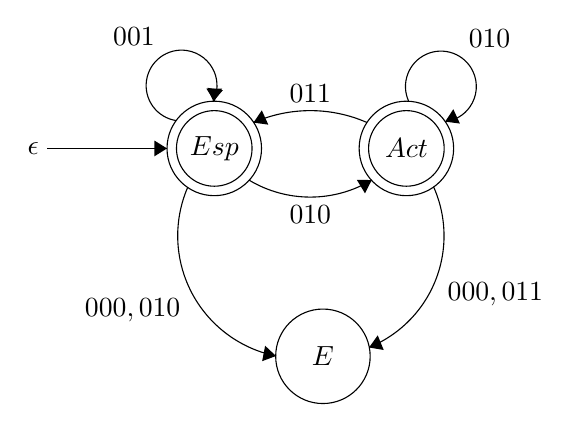
\begin{tikzpicture}[scale=0.2]
	\tikzstyle{every node}+=[inner sep=0pt]
	\draw [black] (37,-18.6) circle (3);
	\draw (37,-18.6) node {$Esp$};
	\draw [black] (37,-18.6) circle (2.4);
	\draw [black] (49.2,-18.6) circle (3);
	\draw (49.2,-18.6) node {$Act$};
	\draw [black] (49.2,-18.6) circle (2.4);
	\draw [black] (43.9,-31.8) circle (3);
	\draw (43.9,-31.8) node {$E$};
	\draw [black] (39.494,-16.958) arc (113.75402:66.24598:8.952);
	\fill [black] (39.49,-16.96) -- (40.43,-17.09) -- (40.02,-16.18);
	\draw (43.1,-15.7) node [above] {$011$};
	\draw [black] (46.998,-20.609) arc (-58.98762:-121.01238:7.566);
	\fill [black] (47,-20.61) -- (46.05,-20.59) -- (46.57,-21.45);
	\draw (43.1,-22.19) node [below] {$010$};
	\draw [black] (37,-15.5) -- (37,-15.6);
	\fill [black] (37,-15.6) -- (37.5,-14.8) -- (36.5,-14.8);
	\draw [black] (34.59,-16.833) arc (261.47443:-26.52557:2.25);
	\draw (31.9,-12.1) node [above] {$001$};
	\fill [black] (36.94,-15.61) -- (37.55,-14.9) -- (36.56,-14.75);
	\draw [black] (26.4,-18.6) -- (34,-18.6);
	\draw (25.9,-18.6) node [left] {$\epsilon$};
	\fill [black] (34,-18.6) -- (33.2,-18.1) -- (33.2,-19.1);
	\draw [black] (50.924,-21.032) arc (24.0977:-67.85012:7.646);
	\fill [black] (46.83,-31.24) -- (47.76,-31.4) -- (47.38,-30.47);
	\draw (51.79,-27.89) node [right] {${000,011}$};
	\draw [black] (40.919,-31.779) arc (-101.43921:-203.36619:7.786);
	\fill [black] (40.92,-31.78) -- (40.23,-31.13) -- (40.04,-32.11);
	\draw (34.88,-28.9) node [left] {${000,010}$};
	\draw [black] (49.35,-15.615) arc (204.86229:-83.13771:2.25);
	\draw (54.48,-12.2) node [above] {$010$};
	\fill [black] (51.66,-16.9) -- (52.6,-17.02) -- (52.18,-16.11);
	\end{tikzpicture}
\end{center}


Podríamos codificar los estados de $Esp$ (espera) y $Act$ (activo) como $000$ y $100$ con lo que tendríamos el estado de error ($E$) codificado como $101$. El autómata describe los posibles pasos en la autenticación de un usuario en un sistema, los estados de 'espera' y 'activo' serían finales dado que son estados 'correctos' en un posible sistema como este. El estado de error, describe justo eso, un comando que no se esperaba dado el estado de la comunicación en el que estábamos. Con este modelo podríamos construir un sistema de autenticación de usuarios usando 3 bits únicamente.
